\documentclass{article}

\usepackage[margin=0.75in, headheight=35pt, includehead, includefoot]{geometry}

\usepackage{fancyhdr}
\usepackage[T1]{fontenc}
\usepackage[shortlabels]{enumitem}
\usepackage{graphicx}
\graphicspath{ {./} }
\usepackage[export]{adjustbox}
\usepackage{booktabs}
\usepackage{forest}
\usepackage{listings}
\lstset{escapeinside={(*@}{@*)}}

\setlength{\parindent}{4em}
\setlength{\parskip}{1em}

\pagestyle{fancy}
\rhead{Alex Kitsul\\230134210\\January 28, 2021}

\begin{document}
\thispagestyle{empty}
\begin{center}
\topskip0pt
\vspace*{\fill}
\Huge Alex Kitsul\\
\Huge 230134210\\
\Huge CPSC 450\\
\Huge Assignment 1 - Report\\
\Huge January 28\\
\vspace*{\fill}
\end{center}
\pagebreak

\section*{Psedocode}
\begin{lstlisting}
main:
	k <- from file
	dna <- from file
	best_k_mer
	
	for all possible (*@\textit{k\_mer}@*) AAA...AA to TTT...TT of length k
	if d(k_mer, dna) < distance(best_k_mer, dna)
		best_k_mer <- k_mer
		
	return best_k_mer
	
d(k_mer, dna):
	total_distance
	for all dna_portions in dna
		current_lowest_distance
		for (*@\textit{i}@*) in the length of (*@\textit{dna\_portion}@*) - length of (*@\textit{k\_mer}@*) + 1
			current_distance
			for (*@\textit{j}@*) in the length of (*@\textit{k\_mer}@*)
				if k_mer[i] does not equal dna_portion[i + j]
					current_distance++
				
			if current_distance < current_lowest_distance
				current_lowest_distance <- current_distance
				
		total_distance += current_lowest_distance
		
	return total_distance
\end{lstlisting}

\pagebreak

\section*{Program Code}
\textbf{\underline{MedianStringProblem.py}}
\begin{lstlisting}
import re
import itertools as it
from Best_K_Mer import Best_K_Mer

def main():
    # Pull in file data
    file_name = input("Enter file name to be evaluated (including file extension): ")
    
    with open(file_name, "r") as input_1:
        try:
            k = int(input_1.readline())
        except:
            print("First line of file does not contain a parseable integer, please
            check file and try again.")
            exit()

        dna_string = input_1.read()
        dna_list = re.split("[\s\n]", dna_string)

        #Have k-mer and list of DNA, now need to iterate through all 
        possible patterns of length k
        letters = ["A", "C", "G", "T"]
        best_k_mer = Best_K_Mer("", -1)

        # Iterates through all possible strings of length k using the letters in "letters"
        for k_mer in it.product(letters, repeat=k):
            distance = d(k_mer, dna_list)
            if distance < best_k_mer.distance or best_k_mer.distance == -1:
                best_k_mer = Best_K_Mer(k_mer, distance)

        # Error handling in case the best_k_mer doesn't update
        if best_k_mer.isNull():
            print("Something went wrong, Best_K_Mer was not updated.")
        else:
            print(best_k_mer.dna)

# Method that calculates the minimum distance for each DNA portion, and returns
  the sum of the distances
def d(k_mer, dna):
    total_distance = 0
    for dna_portion in dna:
        current_lowest_distance = -1
        for i in range(len(dna_portion) - len(k_mer) + 1):
            current_distance = 0
            for j in range(len(k_mer)):
                if (k_mer[j] != dna_portion[i + j]):
                    current_distance += 1
            
            if current_distance < current_lowest_distance or current_lowest_distance == -1:
                current_lowest_distance = current_distance

        # Error handling for if current_lowest_distance doesn't update
        if current_lowest_distance < 0:
            print("Something went wrong, exiting...")
            exit()

        total_distance += current_lowest_distance

    return total_distance

if __name__ == "__main__":
    main()
\end{lstlisting}
\textbf{\underline{Best\_K\_Mer.py}}

\begin{lstlisting}
class Best_K_Mer:
    def __init__(self, dna, distance):
        self.dna = dna
        self.distance = distance

    def isNull(self):
        if self.dna == "" or self.distance == -1:
            return 1
        else:
            return 0
\end{lstlisting}

\pagebreak

\section*{Examples with Output}
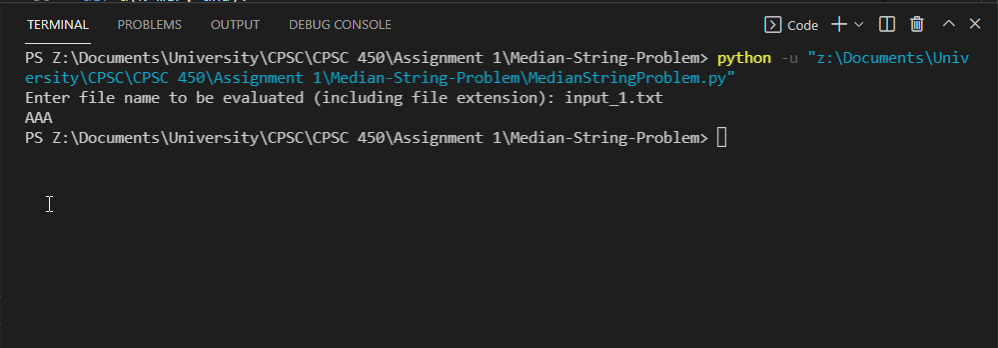
\includegraphics[scale=0.5]{ExampleInput1.png}\\
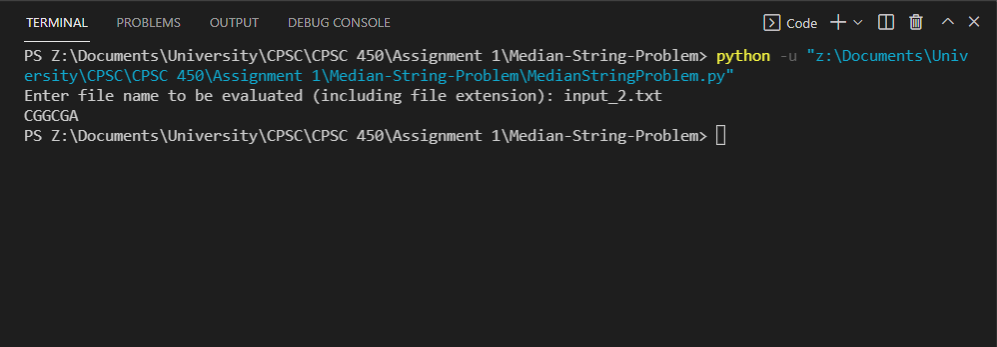
\includegraphics[scale=0.5]{ExampleInput2.png}


\end{document}
